\chapter{Introduction}


\section{Social Network}

\begin{figure}
    \centering
    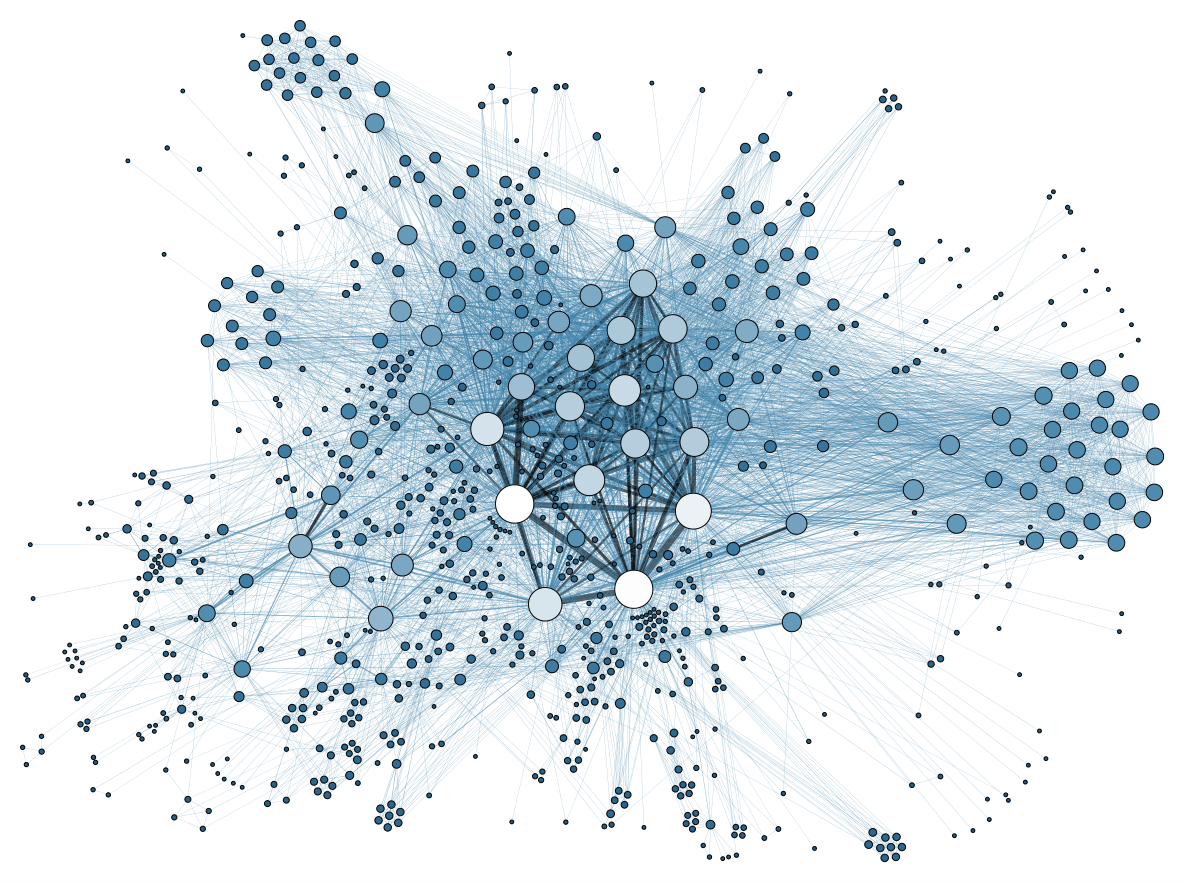
\includegraphics[height=5cm]{tex/img/social_network.png}
    \caption{A social network diagram}
\end{figure}

A \textbf{Social Network} is a network that reflects the social structure of its nodes and their inter-dependency, such as friendship of people, co-authorship of researchers, and collaboration between different parties. Its structure made up of a set of social actors (such as individuals or organizations), sets of dyadic ties, and other social interactions between actors. The scale of a social network is usually very large. The dramatic development in technology has led to more and more people engage in a variety of social activities like chatting, blogging, commenting, and shopping. This has led to researchers having far more questions than answers. 


A social network can be represented and treated as an abstract network of interconnected nodes, and researchers generally adopt a graph or matrix to describe the networks. However, this representation is not scalable. For large social networks, we can expect millions of nodes and edges. It is challenging to decompose or compress such huge graphs. If at all there is a provision to maintain such huge graphs, it is difficult to describe the dynamical features of social networks over such representations. 

\section{Social Influence}

\textbf{Social Influence} is a relationship established between two entities for a specific action. In particular, one entity influences the other entity to perform an action. Usually, the first entity is called the \textit{influencer}, the second entity is called the \textit{influencee}. It is a function of uncertainty because the influence may not have any idea on because the influencee would perform the action. The typical examples are viral marketing, influential bloggers finding, online advertising, social healthcare, expert finding, personalized commendation, citation networks, and so on.


Influence is \textit{asymmetric}: the fact that Alice influences Bob does not necessarily mean that Bob also influences Alice. Influence is \textit{transitive}: if Alice influences Bob and Bob influences Carlos, this implies that Alice influences Carlos indirectly. Influence is \textit{propagative:} information can be passed from one member to another in a social network, creating influence chains. Spreading of influence in social network is the basis of “word of mouth” propagation of information for humans


The research on social influence analysis - still in infancy - interconnects with the other features of social networks, such as influence properties, evaluation metrics of influence, collection and processing social networking big data, and selection of most influential nodes. 


Analyzing social influence helps us: 1) in terms of sociology, it is helpful to understand people’s social behaviors; 2) in terms of public services, it is helpful to provide a theoretical basis for public decision making and public opinion guidance; 3) in terms of political factors, it is helpful to promote national security, economic stability, economic progress, and so on. Hence, social influence analysis is significant and valuable. 
 

There are many challenges in measuring social influence: 1) no mathematical definition; 2) uncertainty; 3) no effective way to integrate external factors; 4) characterizing the relationship.

\begin{figure}
    \centering
    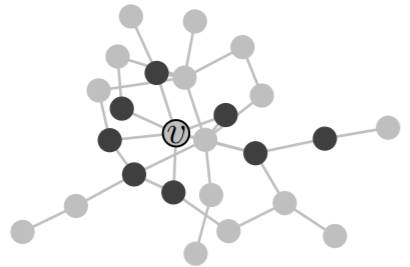
\includegraphics[height=5cm]{tex/img/social_influencer.png}
    \caption{A motivating example of social influence locality prediction}
    \label{fig:influencer}
\end{figure}

In this report, we focus on user level influence - predicting the action status of a user given the action statuses of her near neighbors and her local structural information. For example, in Figure \ref{fig:influencer}, consider vertex $v$ to represent Alice. Suppose her friends Bob, Carlos, and Dave (represented by the black vertices) perform an action, say bought a product, will Alice perform the action in the future?


Researchers have proposed solutions to make such predictions, but they consider complicated hand-crafted features, which require extensive knowledge of specific domains and are usually difficult to generalize to different domains.


\textbf{DeepInf} is an deep learning based end-to-end approach to discover hidden and predictive signals in social influence automatically. Using techniques like network embedding, graph convolution and graph attention mechanism into a unified network, it represents both influence dynamics and network structures in a latent space.

